\documentclass{article}
\usepackage[utf8]{inputenc}
\usepackage{graphicx}
\usepackage{fancyhdr}
\pagestyle{fancy}
\lfoot{\texttt{comsm0094.github.io}}
\lhead{LC\&B - 04.1 Synapses - Conor}
\rhead{\thepage}
\cfoot{}
\begin{document}

\section*{Synapses}

Synapses are what connect neuron to neuron; in this section we look at
how they do this. Next week we will look at how they change their
connection strength in response to activity; plastic changes thought
to underpin learning in the brain.

\subsection*{Chemical synapses}

Spikes, the voltage pulses that carry signals from neuron to neuron,
are notably stereotypical; there aren't big spikes and small spikes,
to a good approximation, there are just spikes. However, the effect
one neuron has on the other can vary considerably, not just from
neuron to neuron, but from time to time. This variablity can occur
because of chemical synapses, the complicated biochemical machinery
responsible for connect the axon of one neuron to the dendrite of
another. 

Chemical synapses are not the only synapses, there are also
\textsl{gap junctions}. If an axon is connected to a dendrite by a gap
junction there is a small hole directly connecting the inside of one
neuron through to the inside of the other, usually this means that the
axon of one neuron is connected to the dentrite of the other, though
axon to axon gap junctions are also found. For an axon to dentrite gap
junction this means that when a spike travelling along the axon
reaches the gap junction some of the charged ions diffuse through the
gap changing the charge in the dendrite. In some simple animals like
jelly fish most or all of the synapses are gap junctions. There are
gap junctions in the mammalian brain, for example gap junctions are
thought to be responsible for the dynamics which supports very rapid
oscillations in the hippocampus, however, most of the synapses in the
mammalian brain are chemical synapses. We will see that this allows a
more variable effect of a pre-synaptic spike on the voltage of the
post-synaptic dendrite.

In a chemical synapse the pre-synaptic spike does not affect the
post-synaptic voltage directly, instead it causes a cascade of
bio-electrodynamics events which ultimately causes a transient change
in conductance of the post-synaptic membrane. 

Roughly, the synapse consists of a protuberance in the axon called the
\textsl{terminal bouton}, the terminal bouton is held by astrocytes,
supporting non-neuronal brain cells, so that it is separated by a tiny
gap, called the \textsl{synaptic cleft} from a protuberance in the
dendrite called the \textsl{dendritic spine}; depending on the neurons
involved this protuberance might be a small bump, or a substantial
spine. Figure~\ref{fig:spines} indicates the range of spine
shapes. The shape of the spine is thought to be important in the
modulation of synaptic signalling; this isn't an aspect of synapses we
will consider here.

\begin{figure}
\begin{center}
$
\begin{array}{lclc}
\textbf{a}&&\textbf{b}&\cr
&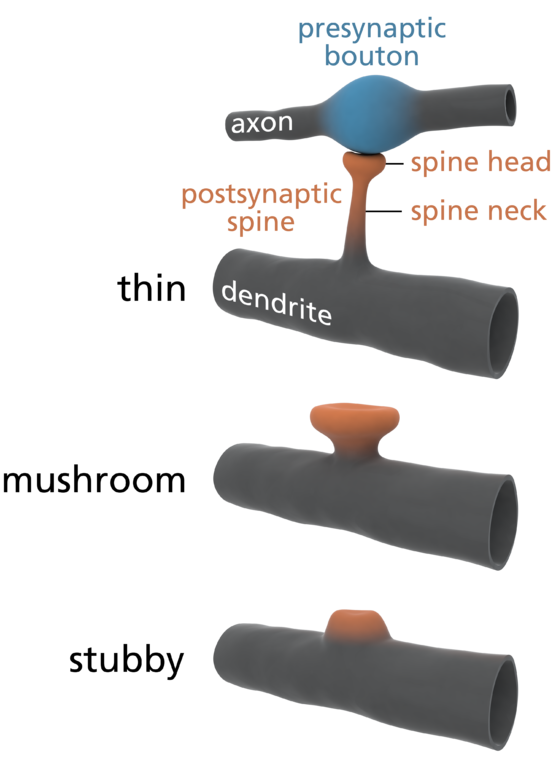
\includegraphics[width=6cm]{Spline_types_3D.png}
&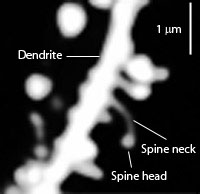
\includegraphics[width=6cm]{Dendritic_spines.jpg}
\end{array}
$
\end{center}
\caption{Types of dendritic spines: \textbf{a} shows a set of different spine types, \textbf{b}
  shows a photograph of a spiny dendrite of a striatal medium spiny
  neuron. [Both pictures from
    \texttt{https://en.wikipedia.org/wiki/Dendritic\_spine}]\label{fig:spines}}
\end{figure}

The terminal bouton is filled with tiny bags or bubbles called
\textsl{vesicles}, these contain special molecules called
\textsl{neurotransmitters}. When a spike arrives at the terminal
bouton it causes calcium gates to open in the cellular membrane, the
resulting influx of calcium ions causes some of the vesicles to
migrate to the membrane separating the bouton from the synaptic cleft,
they burst releasing neurotransmitter into the cleft.

\begin{figure}
\begin{center}
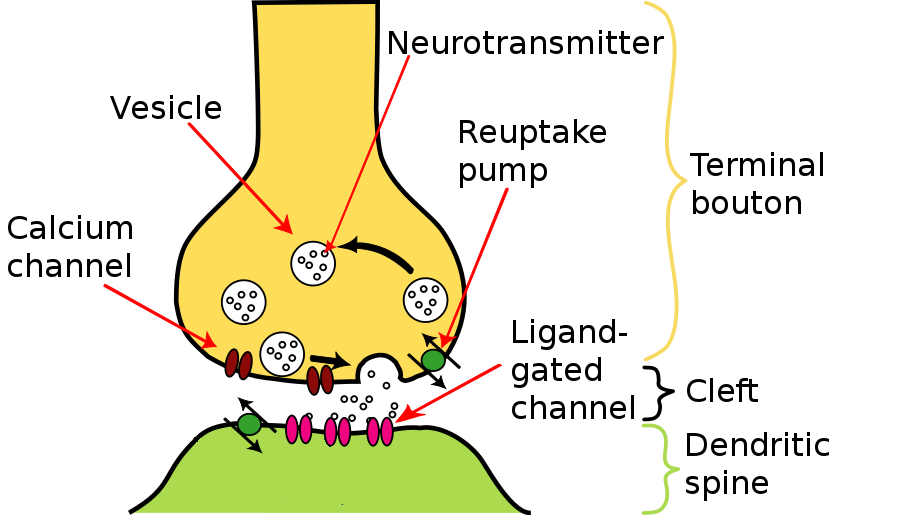
\includegraphics[width=12cm]{Synapse.png}
\end{center}
\caption{The major parts of the synapse; this shows a vesicle
  bursting, releasing neurotransmitter into the cleft, this will bind
  with the ligand-gated channels to allow a current across the
  membrane of the dendrite. Reuptake pumps are shown in the bouton and
  the spine, there are also pumps in the astrocyte that surrounds the
  cleft but isn't shown here. Some is also lost to diffusion. [Diagram
    modified from one in wikipedia.]}
\end{figure}

The membrane of the dendritic is pieced by gated ion channels; these
are \textsl{ligand gated} channels. This means that they contain a
receptor site which binds with a particular type of molecule, like a
key designed for the receptor site's lock. When the receptor has a
molecule bound to it, the gate is open and so ions can pass through
the channel, like the other channels we have seen the channel is ion
specific, so only one type of ion can pass through it. In the case of
the ligand-gated channels in the dendritic spine, the neurotransmitter
binds with the receptor, opening the gate. Hence, after a spike
arrives at the synapse the cleft is filled with neurotransmitter and
some of that neurotransmitter binds to the gated channels, causing
them to open. This in turn allows a flow of ions in or out of the
dendrite, changing the voltage there. A cartoon of a ligand-gated
channel is given in Fig.~\ref{LGIC}.

\begin{figure}
\begin{center}
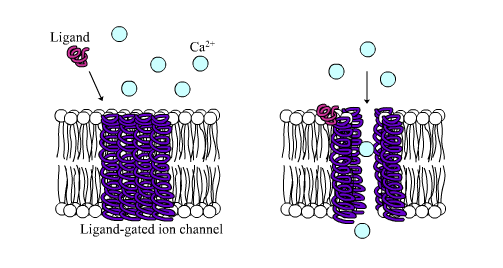
\includegraphics[width=12cm]{LGIC.png}
\end{center}
\caption{Sketch of a ligand-gated channel; when the neurotransmitter,
  the ligand, binds to the gate it opens allowing the ions to pass
  through. This is a Calcium channel, calcium, like sodium, is found
  in higher concentrations outside the cell so the chemical gradient,
  as well as the voltage gradient, means these ions flow into the cell
  from outside, increasing its potential.  This is therefore part of
  an excitatory synapse. Inhibitory synapses have ligand-gated
  potassium and chlorine channels, potassium, as we have discussed, is
  at a higher concentration inside the cell and so will flow out,
  depending on the voltage gradient, lowering the potential inside the
  cell. Chlorine is at a higher concentration outside the cell but is
  a negative ion, so when it flows in it also lowers the
  potential. [Diagram modified from wikipedia.]\label{LGIC}}
\end{figure}

Which ion and which direction, depends on the synapses, we will return
to that. For now, though, let us continue describing what happen;
after the neurotransmitter floods the cleft it is quickly reabsorbed
through neurotransmitter reuptake pumps. Some of the neurotransmitter
is absorbed into the bouton, some into the spine and some is absorbed
by the astrocyte, the important thing is that the concentration of
neurotransmitter in the cleft falls rapidly. Now, the fluid of the
cleft has little neurotransmitter, but there is still neurotransmitter
bound to the receptors of the ligand gated channels. This gradually
unbinds, this is usually imagined to be a random process, because of
the Brownian motion of molecules in the fluid of the cleft and the
thermal vibration of the receptor itself, the neurotransmitters unbind
as the result of random collisions and thermal variations. As they do
so, the channels close again and the conductivity of the dendritic
spine's membrane falls back towards zero.

\subsection*{Post-synaptic potential}

One important property of neurons is that a given neuron is either
\textsl{excitatory} or \textsl{inhibitory}. If a neuron is excitatory,
this means all its synapses are excitatory, that is, they make the
post-synaptic neuron more likely to spike by increasing its
voltage. In an excitatory neuron opening the ligand-gated channels
causes a positive current into the cell, typically this means that
they are sodium or calcium channels, so that when they open positive
sodium or calcium ions flow into the dendrite. Conversely, if a neuron
is inhibitory all its synapses are inhibitory, they make the
post-synaptic cell less likely to fire by decreasing its voltage. In
an inhibitory synapse opening the ligand-gated channels causes a
positive flow out of the dendrite, lowering the voltage. Typically
inhibitory channels are either potassium gates, allowing postive
potassium to leave the dendrite, or chlorine gates, allowing
negatively charged chlorine to flow in.

The post-synaptic change in potential that results from a pre-synaptic
spike is called a \textsl{post-synaptic potential}; if the synapse is
excitatory this is called an \textsl{excitatory post-synaptic
  potential} or EPSP, if it is inhibitory it is called an
\textsl{inhibitory post-synaptic potential} or IPSP. The profile of
PSPs reflects the neurotransmitter dynamics, it rises fast as the
neurotransmitter floods the cleft and the ion-channels open, it then
decays back to zero following an exponential decay, reflecting the
constant rate unbinding process: since any bound molecule has a
constant probability of shaking free the number of unbinding events
depends on the number of bound molecules, giving an exponential decay.

Often the post-synaptic conductivity is taken to be a what is called an
$alpha$ function:
\begin{equation}
I_s(t)=g_ss(t)(E_s-V)
\end{equation}
where $I_s(t)$ is the synpatic current, $E_s$ is the reversal
potential of the synapse and $g_ss(t)$ is the conductance, $g_s$ is a
constant describing the strength of the synapse and $s(t)$ is 
\begin{equation}
s(t)=te^{-t/\tau_s}
\end{equation}
where $\tau_s$ is a time scale, see Fig.~\ref{fig:alpha}. Basically
the rising part of the $\alpha$ function models the period when there
is neurotransmitter in the cleft, this is binding to the channels
increasing the conductance; the falling part represents the period
where the unbound neurotransmitter has been cleared from the cleft and
the bound neurotransmitter is unbinding randomly due to the thermal
motion of molecules. It is possible to understand these dynamics in
terms of the bucket-like equations we have examined before, but this
won't be done here. It is also common to leave out the rising part and
just model the conductance as
\begin{equation}
\tau_s\frac{ds}{dt}=-s
\end{equation}
with
\begin{equation}
s(t)\rightarrow s(t)+1
\end{equation}
whenever there is a spike. This is what is done in the coursework, for
example.

\begin{figure}
\begin{center}
% GNUPLOT: LaTeX picture with Postscript
\begingroup
  \makeatletter
  \providecommand\color[2][]{%
    \GenericError{(gnuplot) \space\space\space\@spaces}{%
      Package color not loaded in conjunction with
      terminal option `colourtext'%
    }{See the gnuplot documentation for explanation.%
    }{Either use 'blacktext' in gnuplot or load the package
      color.sty in LaTeX.}%
    \renewcommand\color[2][]{}%
  }%
  \providecommand\includegraphics[2][]{%
    \GenericError{(gnuplot) \space\space\space\@spaces}{%
      Package graphicx or graphics not loaded%
    }{See the gnuplot documentation for explanation.%
    }{The gnuplot epslatex terminal needs graphicx.sty or graphics.sty.}%
    \renewcommand\includegraphics[2][]{}%
  }%
  \providecommand\rotatebox[2]{#2}%
  \@ifundefined{ifGPcolor}{%
    \newif\ifGPcolor
    \GPcolorfalse
  }{}%
  \@ifundefined{ifGPblacktext}{%
    \newif\ifGPblacktext
    \GPblacktexttrue
  }{}%
  % define a \g@addto@macro without @ in the name:
  \let\gplgaddtomacro\g@addto@macro
  % define empty templates for all commands taking text:
  \gdef\gplbacktext{}%
  \gdef\gplfronttext{}%
  \makeatother
  \ifGPblacktext
    % no textcolor at all
    \def\colorrgb#1{}%
    \def\colorgray#1{}%
  \else
    % gray or color?
    \ifGPcolor
      \def\colorrgb#1{\color[rgb]{#1}}%
      \def\colorgray#1{\color[gray]{#1}}%
      \expandafter\def\csname LTw\endcsname{\color{white}}%
      \expandafter\def\csname LTb\endcsname{\color{black}}%
      \expandafter\def\csname LTa\endcsname{\color{black}}%
      \expandafter\def\csname LT0\endcsname{\color[rgb]{1,0,0}}%
      \expandafter\def\csname LT1\endcsname{\color[rgb]{0,1,0}}%
      \expandafter\def\csname LT2\endcsname{\color[rgb]{0,0,1}}%
      \expandafter\def\csname LT3\endcsname{\color[rgb]{1,0,1}}%
      \expandafter\def\csname LT4\endcsname{\color[rgb]{0,1,1}}%
      \expandafter\def\csname LT5\endcsname{\color[rgb]{1,1,0}}%
      \expandafter\def\csname LT6\endcsname{\color[rgb]{0,0,0}}%
      \expandafter\def\csname LT7\endcsname{\color[rgb]{1,0.3,0}}%
      \expandafter\def\csname LT8\endcsname{\color[rgb]{0.5,0.5,0.5}}%
    \else
      % gray
      \def\colorrgb#1{\color{black}}%
      \def\colorgray#1{\color[gray]{#1}}%
      \expandafter\def\csname LTw\endcsname{\color{white}}%
      \expandafter\def\csname LTb\endcsname{\color{black}}%
      \expandafter\def\csname LTa\endcsname{\color{black}}%
      \expandafter\def\csname LT0\endcsname{\color{black}}%
      \expandafter\def\csname LT1\endcsname{\color{black}}%
      \expandafter\def\csname LT2\endcsname{\color{black}}%
      \expandafter\def\csname LT3\endcsname{\color{black}}%
      \expandafter\def\csname LT4\endcsname{\color{black}}%
      \expandafter\def\csname LT5\endcsname{\color{black}}%
      \expandafter\def\csname LT6\endcsname{\color{black}}%
      \expandafter\def\csname LT7\endcsname{\color{black}}%
      \expandafter\def\csname LT8\endcsname{\color{black}}%
    \fi
  \fi
  \setlength{\unitlength}{0.0500bp}%
  \begin{picture}(5040.00,3528.00)%
    \gplgaddtomacro\gplbacktext{%
      \csname LTb\endcsname%
      \put(1210,704){\makebox(0,0)[r]{\strut{} 0}}%
      \put(1210,1344){\makebox(0,0)[r]{\strut{} 0.001}}%
      \put(1210,1983){\makebox(0,0)[r]{\strut{} 0.002}}%
      \put(1210,2623){\makebox(0,0)[r]{\strut{} 0.003}}%
      \put(1210,3262){\makebox(0,0)[r]{\strut{} 0.004}}%
      \put(1342,484){\makebox(0,0){\strut{} 0}}%
      \put(2002,484){\makebox(0,0){\strut{} 0.02}}%
      \put(2662,484){\makebox(0,0){\strut{} 0.04}}%
      \put(3323,484){\makebox(0,0){\strut{} 0.06}}%
      \put(3983,484){\makebox(0,0){\strut{} 0.08}}%
      \put(4643,484){\makebox(0,0){\strut{} 0.1}}%
      \put(176,1983){\rotatebox{-270}{\makebox(0,0){\strut{}$s(t)$}}}%
      \put(2992,154){\makebox(0,0){\strut{}$t$}}%
    }%
    \gplgaddtomacro\gplfronttext{%
      \csname LTb\endcsname%
      \put(3656,3090){\makebox(0,0)[r]{\strut{}$t\exp{(-t/0.01)}$}}%
    }%
    \gplbacktext
    \put(0,0){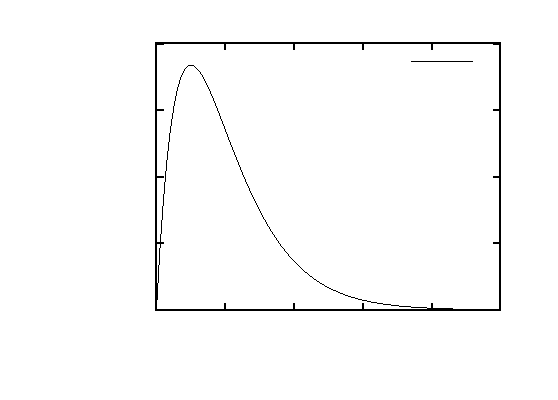
\includegraphics{alpha}}%
    \gplfronttext
  \end{picture}%
\endgroup

\end{center}
\caption{The $\alpha$-function profile often used to model synaptic
  conductances, shown here with $\tau_m=10$ ms.\label{fig:alpha}}
\end{figure}

\subsection*{The complexity of synapses}

The chemical synapse is complicated and there are many details of the
synapse that can effect the dynamics. For example, the strength of the
synapse, that is, the amplitude of the change in conductance that
follows a pre-synaptic spike, depends on the number of vesicles
released, on the size of the cleft, the speed of reuptake and the
number of ligand-gated channels; the shape and duration of the PSP
depends on the detailed dynamics of binding, reuptake and unbinding
and the effect of the PSP on the post-synaptic soma depends on the
shape of the dendritic tree and the details of the diffusive process
which conducts the PSP to the soma, a distal synapse will have a
different effect to a proximal one. The shape of the dendritic spine
can also filter the PSP, modulating its shape.

Some aspects of synaptic dynamics vary from synapse to synapse;
usually the length of a timescale depends on the neurotransmitter and
receptor; excitatory synapses tend to have shorter time constants than
inhibitory ones, but excitatory synapses have two common receptors for
glutamate, the most common excitatory transmitter: NMDA-receptors
which are quick and AMPA receptors, which are slow. In the case of
inhibitory synapses the most common transmitter is called GABA and the
common receptors are the simpler GABA-A receptor and the more
complicated GABA-B receptors. We will see that some special synapses
release neuromodulators rather than neurotransmitters; these often
change behaviors in subtler ways.

There are typically spike-to-spike effects usually described as
\textsl{short term plasticity}, for example if two spikes arrive one
soon after the other, the first might have already opened a
substantial quantity of the gates, reducing the effect of the second.
If there is a high rate of pre-synaptic spike arrivals the vesicles
may be depleted reducing the size of PSPs, this is called
\textsl{short term depression}; sometimes the opposite is true, the
build up of calcium ions in response to a high rate of pre-synaptic
spiking can increase the size of PSPs, this is \textsl{short term
  facilitation}. Short term plastic effects, with timescales of 10 ms
up to seconds are thought to play an important role in neural
computation \cite{AbbottEtAl1997a}. This short term plasticity is
usually distinguished from \textsl{long term plasticity}, the long term changes
in the structure of the synapses that are thought to be responsible
for learning and development in the brain. Long term plasticity will be considered next.

\begin{thebibliography}{10}

\bibitem{AbbottEtAl1997a}
Abbott LF, Varela JA, Sen K and Nelson SB. (1997) Synaptic depression and cortical gain control. 
\newblock Science, 275: 221--224.

\end{thebibliography}

\end{document}
